\section{Extension of the moving-pair tensors}
\label{ext:section}

Fix the degree-two very free map $g:\PP^1\to X$ supplied by
Proposition~\ref{sm:very-free}. We continue in the primitive Picard
case. The construction in this section uses only the ampleness of $L$,
the contact form, and this one map with its two-point evaluation
property. Both points on the source will vary.

Write $\operatorname{pr}_i:X\times X\to X$ for the projections and set
\[
\mathcal E_{12}=T_X\boxtimes L,\qquad
\mathcal E_{21}=L\boxtimes T_X,\qquad
\mathcal M_X=L\boxtimes L.
\]
The contact form induces maps $\mathcal E_{12}\to\mathcal M_X$ and
$\mathcal E_{21}\to\mathcal M_X$.

\begin{proposition}[The proper moving-pair construction]
\label{ext:moving-pair}
There are a proper integral algebraic space $Y$, a dominant morphism
$p:Y\to X\times X$, and sections
\[
W_{12}\in H^0(Y,p^*\mathcal E_{12}),\qquad
W_{21}\in H^0(Y,p^*\mathcal E_{21})
\]
with common contact value
\[
\xi=(\theta\boxtimes 1)(W_{12})
     =(1\boxtimes\theta)(W_{21})
\in H^0(Y,p^*\mathcal M_X).
\]
There is an involution $\iota$ of $Y$ over the interchange of the two
factors of $X\times X$, under which $\xi$ is invariant using the
canonical interchange of the line factors.

Moreover, for a full open neighborhood $\mathcal H$ of $g$ in
$\operatorname{Hom}_2(\PP^1,X)$ there is a morphism
\[
j:\mathcal H\times\PP^1\times\PP^1\longrightarrow Y,
\qquad p(j(h,z,w))=(h(z),h(w)).
\]
In an affine coordinate containing $z,w$, its pullbacks satisfy
\begin{equation}\label{ext:hom-vectors}
\begin{aligned}
j^*W_{12}(h,z,w)
  &=(z-w)^2h'(z)\otimes\theta(h'(w)),\\
j^*W_{21}(h,z,w)
  &=(z-w)^2\theta(h'(z))\otimes h'(w),
\end{aligned}
\end{equation}
and hence
\begin{equation}\label{ext:hom-identity}
j^*\xi(h,z,w)
  =(z-w)^2\theta(h'(z))\otimes\theta(h'(w)).
\end{equation}
These formulas are independent of the coordinate.
\end{proposition}

We construct the two vector sections first on the universal square over
smooth sources. Normality then reduces their extension to boundary
divisors (Lemma~\ref{ext:normal-products}). A singular unmarked
degree-two source has two components. At a node of
thickness $r$, the contact differential vanishes to order at least $r$
(Lemma~\ref{ext:contact-order}), while the tensor has a pole of order at
most $r$ on the mixed products, as in Equation~\eqref{ext:pole-table}.
One contact factor therefore extends each vector lift. Passing to the coarse
space then gives $Y$ and the full family.

\subsection{The normalized component and its universal-curve square}

Let $\beta$ be the numerical curve class specified by the degree
functional of $g$ on $\operatorname{Pic}(X)$, as in the convention
of Behrend--Manin. Since $\operatorname{Pic}(X)=\ZZ[L]$, fixing
$L$-degree two fixes this functional. The stable-map
Theorem gives a proper Deligne--Mumford stack of finite type
\[
\overline{\mathcal M}_{0,0}(X,\beta).
\]
Here the target is smooth and projective, the class is nonzero, and the
ground field has characteristic zero. These are the applicable
hypotheses of \cite[Theorem~3.14 and Corollary~4.8]{BM1996}; in
characteristic zero the characteristic bound in Theorem~3.14 is
automatic. The number of stability markings is zero. Its universal
source is a proper flat family of geometrically connected nodal
curves of arithmetic genus zero, with its universal map to $X$.
The universal-curve statement also follows from
\cite[Corollary~4.6]{BM1996}.

By Lemma~\ref{sm:full-germ}, the stack is smooth at $[g]$ and has a
unique irreducible component there. Give this closed component its reduced structure and
normalize it, obtaining $\mathcal S$. The normalization is finite:
on an \emph{\'etale} scheme atlas, the component is of finite type over
$\CC$, hence Nagata, and its normalization is finite. These
normalizations agree under \'etale base change and therefore descend
to the stack \cite[Tags \stacksTag{0GMJ}, \stacksTag{035B}, and \stacksTag{035S}]{Stacks}.
Consequently $\mathcal S$ is proper, integral and normal. The
normalization is an isomorphism on a full smooth neighborhood of
$[g]$.

Pull back the universal source and form its fiber square:
\begin{equation}\label{ext:universal}
\pi:\mathcal C\longrightarrow\mathcal S,\qquad
e:\mathcal C\longrightarrow X,\qquad
\mathcal D=\mathcal C\times_{\mathcal S}\mathcal C,
\qquad \widetilde p=(e_1,e_2):\mathcal D\longrightarrow X\times X.
\end{equation}
These are proper Deligne--Mumford stacks. On scheme charts the source
families are projective: if $A_X$ is an ample line bundle on $X$, then
$\omega_\pi\otimes e^*A_X^{\otimes k}$ has positive degree on every
source component for sufficiently large $k$, by stability, and is a
relative polarization. In particular all the proper-curve arguments
below take place on schemes after passing to such charts.

The points of $\mathcal D$ select two points on the \emph{unmarked}
source. They may coincide and they may be nodes. They do not add
stability markings to that source. The identification of a universal
curve with a moduli stack having one more marking uses stabilization
at a node; it does not change the fiber of the universal curve used
in \eqref{ext:universal}.

By Lemma~\ref{sm:full-germ}, a full open neighborhood $\mathcal H$ of
$g$ in the parametrized Hom scheme maps to $\mathcal S$, and the
source pulled back there is $\mathcal H\times\PP^1$. It therefore
gives a morphism
\begin{equation}\label{ext:hom-to-stack}
\widetilde j:\mathcal H\times\PP^1\times\PP^1
\longrightarrow\mathcal D.
\end{equation}
Two-point evaluation at $g$ is submersive by
Proposition~\ref{sm:very-free}. Its factorization through
$\widetilde p$ proves that $\widetilde p$ is dominant. In particular,
this construction retains the entire nearby parametrized family.

\subsection{The invariant tensor on smooth sources}

On $\PP^1\times\PP^1$ define
\begin{equation}\label{ext:bivector}
\mathfrak b(z,w)=(z-w)^2\partial_z\otimes\partial_w
\in H^0(\PP^1\times\PP^1,T_{\PP^1}\boxtimes T_{\PP^1}).
\end{equation}
For a fractional-linear coordinate change $T$ one has
\[
(T(z)-T(w))^2=(z-w)^2T'(z)T'(w).
\]
This proves coordinate independence and regularity at infinity.
The tensor vanishes to order two on the diagonal and is unchanged
by simultaneous reparametrization. A smooth proper family of
genus-zero curves admits parametrizations locally in the smooth
topology; the displayed invariance therefore descends the tensor
algebraically to its relative square. It also accounts for every
finite automorphism of a stable map, including a possible deck
transformation of a multiple cover.

Let $\mathcal S^\circ\subset\mathcal S$ be the nonempty open of smooth
sources, and put $\mathcal D^\circ=\mathcal D|_{\mathcal S^\circ}$.
On this open stack define
\begin{equation}\label{ext:initial-vectors}
\begin{aligned}
W_{12}^{\circ}
  &=(d_\pi e_1\otimes\theta d_\pi e_2)(\mathfrak b)
    \in H^0(\mathcal D^\circ,\widetilde p^*\mathcal E_{12}),\\
W_{21}^{\circ}
  &=(\theta d_\pi e_1\otimes d_\pi e_2)(\mathfrak b)
    \in H^0(\mathcal D^\circ,\widetilde p^*\mathcal E_{21}).
\end{aligned}
\end{equation}
Here the relative differentials are taken in the two source
variables. Their contact values agree and are invariant under
interchange of those variables. We will extend the \emph{vector}
sections in \eqref{ext:initial-vectors}.

\subsection{Normality and the divisors to be checked}

The formulas above define sections on the smooth-source open. We now
prove that $\mathcal D$ is integral and normal, so these sections are
rational sections and their extension can be checked at divisors.

\begin{lemma}[Normality and the divisorial points]
\label{ext:normal-products}
Let $B$ be a normal integral locally Noetherian scheme, and let
$C_i\to B$, for $1\leq i\leq k$, be flat nodal-curve families of
finite presentation. Suppose the \emph{entire} generic fiber of each
family is smooth and geometrically integral. Then
$P=C_1\times_B\cdots\times_B C_k$ is integral and normal.
Every height-one point of $P$ lies either over the generic point of
$B$, or at a generic point of a fiber component over a height-one
point of $B$. In the latter case every selected point of every
$C_i$ is relatively smooth.
\end{lemma}

\begin{proof}
The morphism $P\to B$ is flat and of finite presentation. Its fibers
are geometrically reduced and are local complete intersections:
\'etale locally, a product of nodal curves is cut out by nodal
equations in disjoint sets of variables. They are therefore
Cohen--Macaulay. Their component generic points are smooth over the
residue field. These assertions also follow from the syntomic
description of nodal families and its stability under base change
and composition \cite[Tags \stacksTag{0C59}, \stacksTag{01UH}, and \stacksTag{01UI}]{Stacks}.

For reducedness, on affine charts flatness over the domain defining
an affine open of $B$ makes the coordinate algebra inject into its
generic localization. The latter is reduced, since the entire
generic fiber is smooth. Thus the total space is reduced.
Every nonempty open of $P$ has nonempty open image in $B$, by
flatness and finite presentation, so it meets the generic fiber.
Two such opens intersect on that geometrically integral fiber.
Hence $P$ is irreducible and therefore integral.

For Serre's condition $S_2$, use the following flat ascent statement:
a flat homomorphism of Noetherian rings whose base and fiber rings
are $S_2$ has $S_2$ total ring
\cite[Lemma~10.163.4, Tag \stacksTag{0339}]{Stacks}. The normal base is $S_2$
and our fibers are Cohen--Macaulay, so the statement applies.
If $q\in P$ has height one and maps to $b\in B$, the flat local
dimension formula \cite[Tag \stacksTag{00ON}]{Stacks} gives
\[
1=\dim\OO_{P,q}
 =\dim\OO_{B,b}+\dim\OO_{P_b,q}.
\]
If $b$ is generic, $\OO_{P,q}$ is regular because the entire
generic fiber is smooth. Otherwise $b$ has height one,
$\OO_{B,b}$ is a DVR, and $q$ is a component generic point of the
fiber. All its coordinates are then smooth points of the nodal
fibers. The product morphism is smooth there, so its total space is
regular over the regular local base. This proves $R_1$.
Serre's criterion now gives normality
\cite[Tag \stacksTag{031S}]{Stacks}, and also proves the claimed description of
height-one points.
\end{proof}

The hypothesis about the generic fiber in
Lemma~\ref{ext:normal-products} is stronger than generic smoothness
of the individual fibers. It is satisfied here: $\mathcal S^\circ$ contains $[g]$, so it is a nonempty open
in the integral stack $\mathcal S$. On every integral normal \'etale chart of $\mathcal S$, the
entire generic source is a smooth geometrically integral genus-zero
curve. Lemma~\ref{ext:normal-products} applies for $k=1,2$ and proves normality of
$\mathcal C$ and $\mathcal D$. Their global irreducibility can also
be checked directly: the images of two nonempty opens under their
flat structure maps intersect in $\mathcal S^\circ$, and the two
opens then intersect on its geometrically integral fiber. Thus both
stacks are integral.

In particular, no height-one point of $\mathcal D$ lies over a base
stratum of codimension at least two. Over a base divisor it must be
a generic point of a product of source components. A point selecting
a node in either factor cannot be such a generic point. These facts
specify exactly the divisors that must be checked for extension.

\subsection{The unmarked boundary and its contact order}

\begin{lemma}[The degree-two source trees]\label{ext:trees}
A geometric source of an unmarked stable map of genus zero and
$L$-degree two is either smooth, or is exactly two copies $A,J$ of
$\PP^1$, joined at one node, with $L$-degree one on each. There are
no contracted components.
\end{lemma}

\begin{proof}
The dual graph of a connected nodal curve of arithmetic genus zero
is a tree, and every component is a smooth rational curve. Ampleness
of $L$ gives positive integral degree on every nonconstant component,
so there are at most two such components. A contracted component
must have at least three incident nodes for unmarked stability;
in particular every leaf is nonconstant. A nontrivial tree has at
least two leaves. There must therefore be exactly two leaves, each
of degree one, and the tree is a path. All its possible interior
vertices would be contracted of valence two and thus unstable.
There are none. A one-vertex tree is a smooth rational source of
degree two.
\end{proof}

By normality, it suffices to extend at height-one points, since the
two target bundles in \eqref{ext:initial-vectors} are locally free
on all of $\mathcal D$. The only unexamined points lie over divisors
of $\mathcal S$ with singular source. Take the corresponding DVR
$R_0$ on an integral normal \'etale scheme chart of $\mathcal S$.
For computing valuations we may pass to its completed strict
henselization $R$. This is a faithfully flat DVR extension with
algebraically closed residue field $k$ of characteristic zero.
Write $\tau$ for a uniformizer. The special components and node
are now split. Regularity at their generic points is detected after
this replacement: both before and after it the local rings are
DVRs, and $\tau$ has order one because the special fibers are
reduced. A pole would retain its negative valuation on a component
above it.

Let $C\to\operatorname{Spec}R$ be the pulled-back source and retain
the notation $e:C\to X$. Its entire generic fiber is smooth and
geometrically integral. Lemma~\ref{ext:normal-products}, which also
applies to this Noetherian DVR base, makes $C$ and $C\times_R C$
integral and normal. By Lemma~\ref{ext:trees},
$C_k=A\cup J$ with one node $o$. The completed local ring at $o$ is
\begin{equation}\label{ext:node}
\widehat{\OO}_{C,o}\simeq
Q:=R[[u,v]]/(uv-\tau^r),\qquad r\geq1,
\qquad A=(v,\tau),\quad J=(u,\tau).
\end{equation}
Indeed the nodal local-form Lemma assumes a locally finite-type
map, a Noetherian local base, flatness at the point, and a split
node in the fiber; all hold here
\cite[Lemma~53.20.11, Tag \stacksTag{0CBX}]{Stacks}. Its smoothing parameter is
nonzero since the generic fiber is smooth; write it as a unit times
$\tau^r$ and absorb the unit into one coordinate. We do not assume
that the total space is regular at $o$ or that the individual special
components are Cartier.

Figure~\ref{fig:unmarked-boundary} records the source geometry and the
role of the two evaluation points.
\begin{figure}[H]
\centering
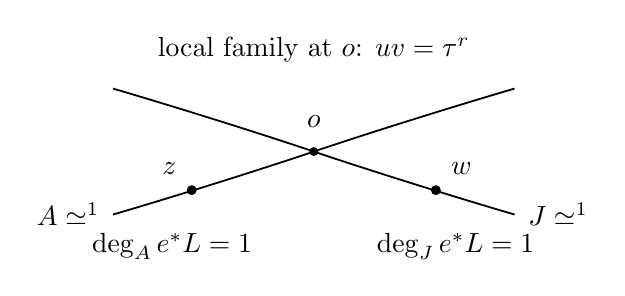
\begin{tikzpicture}[x=1cm,y=1cm,>=stealth]
  \draw[line width=0.65pt] (-2.55,-.80) .. controls (-1.7,-.55) and
    (-.65,-.22) .. (0,0) .. controls (.65,.22) and (1.7,.55) .. (2.55,.80);
  \draw[line width=0.65pt] (-2.55,.80) .. controls (-1.7,.55) and
    (-.65,.22) .. (0,0) .. controls (.65,-.22) and (1.7,-.55) .. (2.55,-.80);
  \node[anchor=east] at (-2.60,-.80) {$A\simeq\PP^1$};
  \node[anchor=west] at (2.60,-.80) {$J\simeq\PP^1$};
  \node at (-1.8,-1.20) {$\deg_A e^*L=1$};
  \node at (1.8,-1.20) {$\deg_J e^*L=1$};
  \fill (0,0) circle (1.6pt);
  \node[above=5pt] at (0,0) {$o$};
  \fill (-1.55,-.49) circle (1.8pt);
  \node[above left=2pt] at (-1.55,-.49) {$z$};
  \fill (1.55,-.49) circle (1.8pt);
  \node[above right=2pt] at (1.55,-.49) {$w$};
  \node at (0,1.30) {local family at $o$: $uv=\tau^r$};
\end{tikzpicture}
\caption{The split special source $A\cup J$, shown schematically.
The two crossing curves represent the rational components of contact
degree one. Their square has component types $A\times A$, $A\times J$,
$J\times A$ and $J\times J$.
The displayed pair $(z,w)$ lies in the mixed component $A\times J$
of the source square; this is one of the two component types where
the bivector may have a pole. The evaluation points are not stability
marks: either may also lie at the node, and they may coincide.
The picture represents the source curve, not its image in $X$.
The bounds in Equation~\eqref{ext:pole-table} and the contact vanishing
of Lemma~\ref{ext:contact-order} explain the cancellation.}
\label{fig:unmarked-boundary}
\end{figure}


\begin{lemma}[Contact vanishing at a boundary trait]
\label{ext:contact-order}
On the relatively smooth locus at the generic point of either $A$
or $J$, the bundle map
$\theta d_\pi e:T_{C/R}\to e^*L$ is divisible by $\tau^r$.
\end{lemma}

\begin{proof}
Nodal fibers are Gorenstein curves. Thus $\omega_{C/R}$ is an
invertible sheaf and its formation commutes with base change
\cite[Tag \stacksTag{0E6R}]{Stacks}. Put
\[
\mathcal N=e^*L\otimes\omega_{C/R}.
\]
On either special component the dualizing degree is $-2+1=-1$,
so $\mathcal N$ has multidegree $(0,0)$. Trivializations on $A$ and
$J$ can be rescaled to agree at their common node. Hence
$\mathcal N|_{C_k}\simeq\OO_{C_k}$, with $h^0=1$ and $H^1=0$.
On the geometric generic rational curve its degree is $2-2=0$,
so its geometric generic restriction is trivial as well.

We spell out the needed cohomology and base change over $R$.
For any line bundle $\mathcal Q$ on $C$ with
$H^1(C_k,\mathcal Q|_{C_k})=0$, multiplication by $\tau$ gives
\[
0\longrightarrow\mathcal Q\xrightarrow{\ \tau\ }
\mathcal Q\longrightarrow\mathcal Q|_{C_k}\longrightarrow0.
\]
Proper coherent cohomology is finite over the Noetherian ring $R$
\cite[Section~30.19, Tag \stacksTag{02O3}]{Stacks}. The long exact sequence
and Nakayama's Lemma therefore give $H^1(C,\mathcal Q)=0$ and
\begin{equation}\label{ext:dvr-base-change}
H^0(C,\mathcal Q)/\tau H^0(C,\mathcal Q)
\simeq H^0(C_k,\mathcal Q|_{C_k}).
\end{equation}
The finite module $H^0(C,\mathcal Q)$ is torsion-free, hence free
over $R$. Its localization is the space of sections on the generic
fiber by flat base change \cite[Section~30.5, Tag \stacksTag{02KE}]{Stacks}.
If $\mathcal Q|_{C_k}$ is globally generated, the evaluation
cokernel vanishes on the special fiber by
\eqref{ext:dvr-base-change} and Nakayama. Its support is proper
over $R$, so if nonempty it would meet the special fiber. Thus
evaluation is surjective everywhere.

Apply this to $\mathcal N$. Its pushforward is free of rank one,
and evaluation is a surjection between line bundles and hence an
isomorphism. In particular there is a nowhere-vanishing global
generator $m$ of $\mathcal N$.

The pullback of the contact form, followed by the natural
differential-to-dualizing map, is
\[
e^*L^{-1}\longrightarrow\Omega^1_{C/R}
\longrightarrow\omega_{C/R}.
\]
Equivalently it is a section $\eta$ of $\mathcal N$. There is
therefore a scalar $h_R\in R$ such that
\begin{equation}\label{ext:eta}
\eta=h_Rm.
\end{equation}
After completing the coherent map $\Omega^1_{C/R}\to\omega_{C/R}$ at
the node, a dualizing generator in $Q$ is represented by
$\gamma=du/u=-dv/v$. The canonical map sends
$du$ to $u\gamma$ and $dv$ to $-v\gamma$. This follows either
from the hypersurface dualizing formula or by checking on the two
smooth coordinate charts; the expressions respect
$v\,du+u\,dv=0$ and extend in the invertible dualizing sheaf.
In a local frame of $e^*L$, the coefficient of $\eta$ consequently
belongs to $(u,v)\subset Q$. Write $m=c$ times the product of this
frame with $\gamma$, where $c\in Q^\times$. The coefficient of
$\eta=h_Rm$ is $h_Rc$; multiplying by $c^{-1}$ preserves the ideal
$(u,v)$. Thus \eqref{ext:eta} implies
\begin{equation}\label{ext:ideal-intersection}
h_R\in (u,v)\cap R=(\tau^r).
\end{equation}
The ideal intersection is exact: $Q/(u,v)=R/(\tau^r)$.
At either component generic point, $m$ is a unit and $\tau$ has
order one. Moreover $\Omega^1_{C/R}\to\omega_{C/R}$ is an
isomorphism there, since that point is relatively smooth. Thus
\eqref{ext:ideal-intersection} gives the claimed order for the actual
contact differential on both components.
\end{proof}

\subsection{A contraction and the possible tensor poles}

To measure the possible poles of $\mathfrak b$, we identify the generic
source with $\PP^1$ by a morphism that preserves one special component
and contracts the other. The invariant tensor on $\PP^1$ is regular.
Transporting it to the source uses the inverse differential of this
morphism, whose vanishing orders will therefore bound the poles.

Choose a $k$-point of $A\setminus\{o\}$. Smoothness at that point
and henselianity give a section $\sigma:\operatorname{Spec}R\to C$
through it. Its image lies in the relatively smooth locus and is a
Cartier divisor. The line bundle $\OO_C(\sigma)$ has multidegree
$(1,0)$ on $A\cup J$. Its sections on $A$ extend uniquely as constant
sections on $J$ with matching value at $o$. This proves global
generation, $h^0=2$, and $H^1=0$ on the special fiber, for example
by the normalization sequence. The argument
\eqref{ext:dvr-base-change} gives a free rank-two pushforward and
surjective evaluation on $C$. Choosing a basis defines
\begin{equation}\label{ext:contraction}
\phi:C\longrightarrow\PP^1_R.
\end{equation}
It is an isomorphism on $A$ and contracts $J$. On the generic fiber
the line bundle has degree one, and its complete linear system is
an isomorphism to $\PP^1_{\operatorname{Frac}(R)}$: this may be
checked after an algebraic closure and then descended. Thus no
split-conic assumption on the original generic source was needed.

The differential of \eqref{ext:contraction}, composed with
$\Omega^1_{C/R}\to\omega_{C/R}$, is a section
\[
\delta_\phi\in H^0(C,\mathcal M),\qquad
\mathcal M=\omega_{C/R}\otimes\phi^*T_{\PP^1_R/R}.
\]
It is nowhere zero on the entire generic fiber, because $\phi$ is
an isomorphism there. Its zero divisor is therefore effective and
vertical. Write its Weil divisor on the normal surface $C$ as
\begin{equation}\label{ext:differential-divisor}
\operatorname{div}(\delta_\phi)=b_AA+b_JJ.
\end{equation}
At the generic point of $A$ the ordinary differential of $\phi|_A$
is nonzero, so $b_A=0$.

\begin{lemma}[The contracted-component order]
\label{ext:differential-order}
With the notation above, $b_J=r$.
\end{lemma}

\begin{proof}
Set $b=b_J$ and normalize the generic order along $J$ first:
\[
\delta'=\tau^{-b}\delta_\phi.
\]
This rational section has order zero in the component DVR of $J$.
It therefore has a well-defined nonzero \emph{generic restriction}
$s_J$ to $J$, a rational section of $\mathcal M|_J$. This operation
means reduction of a unit in that DVR, and is not the usual residue
of a meromorphic differential. At any point of $J\setminus\{o\}$,
the local Weil divisor of $\delta'$ is zero. In a local line frame,
its coefficient and inverse are regular by normality, so $s_J$ has
neither zero nor pole there. Its divisor on $J$ is supported at $o$.

We compute the order at $o$ without restricting a section having a
pole along $J$. First the completed local ring $Q$ in
\eqref{ext:node} is normal. It is a hypersurface over a regular
complete DVR, hence Cohen--Macaulay. A prime containing both $u,v$
also contains $\tau$ and is the height-two maximal ideal. Thus at a
height-one prime one of $u,v$ is invertible, and the hypersurface is
regular there, as its corresponding partial derivative is a unit.
Serre's criterion proves normality; as a local normal ring it is a
domain. In this ring,
\begin{equation}\label{ext:local-divisors}
\operatorname{div}(v)=rA,\qquad
\operatorname{div}(\tau)=A+J.
\end{equation}
For example, at the generic point of $A$, $u$ is a unit and
$v=\tau^r/u$; on $J$, $v$ is a unit. There are no horizontal
components in the divisor of $v$, since $uv=\tau^r$.

Choose a frame of $\mathcal M$ in the local ring
$\OO_{C,o}$, and let $a$ be the coefficient of $\delta_\phi$.
Since $\delta_\phi$ is nowhere zero on the entire generic fiber,
$a$ and $a^{-1}$ belong to $\OO_{C,o}[1/\tau]$. Their images are
therefore units of $Q[1/\tau]$: every height-one prime of $Q$
avoiding $\tau$ has valuation zero on $a$. In particular completion
introduces no horizontal zero or pole. The two height-one primes containing $\tau$
are the component primes $A$ and $J$. Their DVRs dominate the
corresponding component DVRs of $\OO_{C,o}$, with $\tau$ of order
one in both rings because the special fibers are reduced. A local
expression $a=\tau^j a_0$ with $a_0$ a unit therefore retains its
order $j$, since the image of $a_0$ is still a unit.
Consequently, for the coefficient $f=\tau^{-b}a$ of $\delta'$ in
the completed frame,
\[
\operatorname{div}_Q(f)=-bA.
\]
It follows from \eqref{ext:local-divisors} that $f^rv^b$ has zero
valuation at every height-one prime of $Q$. A normal Noetherian
domain is the intersection of its height-one local rings inside
its fraction field \cite[Tag \stacksTag{031T}]{Stacks}. Applying this to both
the function and its inverse gives
\begin{equation}\label{ext:unit-equation}
f^r=v^{-b}\varepsilon,\qquad \varepsilon\in Q^\times.
\end{equation}

Now reduce \eqref{ext:unit-equation} at the generic point of $J$.
This reduction is legitimate because $f$ has order zero there.
The image of $v$ is a parameter on the smooth curve $J$ at $o$,
and the image of $\varepsilon$ is a unit of $k[[v]]$. Hence
$s_J^{\otimes r}$ has order $-b$ at $o$. It has no other zero or
pole. On the other hand,
\[
\deg(\mathcal M|_J)
 =\deg(\omega_{C/R}|_J)
   +\deg(\phi^*T_{\PP^1_R/R}|_J)=-1+0=-1.
\]
The degree of the divisor of $s_J^{\otimes r}$ is therefore $-r$.
Thus $-b=-r$, proving $b_J=r$. The proof only used the Weil
divisors of the components; it did not assume that $A$ or $J$ is
Cartier when $r>1$.
\end{proof}

\subsection{The four product components and extension}

The special fiber of $C\times_R C$ has the four irreducible
components
\[
A\times A,\qquad A\times J,\qquad
J\times A,\qquad J\times J,
\]
where products in this display are over $k$. At each of their
generic points both source variables are relatively smooth. Thus
there are two ordinary relative tangent lines in which to measure
the order of $\mathfrak b$. The local ring of the product at such
a generic point is a DVR with uniformizer $\tau$. Pullback from a
component generic point of $C$ preserves order, since it sends
$\tau$ to this same uniformizer and a unit to a unit.

On the generic fiber, invariance of the canonical tensor gives
\begin{equation}\label{ext:contracted-bivector}
(d\phi\otimes d\phi)(\mathfrak b)
  =(\phi\times\phi)^*\mathfrak b_{\PP^1_R}.
\end{equation}
The right-hand side is regular. At these relatively smooth points,
the component orders of $d\phi$ are the orders of $\delta_\phi$:
they are $0$ on $A$ and $r$ on $J$, by
Lemma~\ref{ext:differential-order}. Inverting the two differentials
in \eqref{ext:contracted-bivector} therefore costs no order on
$A\times A$, and at most $r$ on either mixed component. For
$J\times J$, repeat the construction with a section through a
smooth point of $J$, obtaining a contraction that preserves $J$
and contracts $A$. Both differential orders on $J\times J$ are
then zero. Altogether the bounds are
\begin{equation}\label{ext:pole-table}
\begin{array}{c|cccc}
\text{component}&A\times A&A\times J&J\times A&J\times J\\ \hline
\operatorname{ord}(\mathfrak b)\text{ at least}
 &0&-r&-r&0.
\end{array}
\end{equation}
Each same-component product uses a contraction preserving that
component. On each mixed product, exactly one inverse differential
contributes a possible pole of order $r$.

Lemma~\ref{ext:contact-order} supplies order at least $r$ for the
contact differential in \emph{either} variable. For $W_{12}^\circ$
use the contact differential in the second variable, and for
$W_{21}^\circ$ use it in the first. In each case this cancels the
only possible negative order in \eqref{ext:pole-table}. The remaining
ordinary differential $d_\pi e$ is a regular homomorphism at these
relatively smooth generic points. Thus each vector section has
nonnegative order on all four product components.

We have checked every height-one point not already in
$\mathcal D^\circ$. On a normal Noetherian scheme, a rational
section of a locally free sheaf which is regular at all height-one
points is regular everywhere: trivialize the sheaf and use the
normal-domain intersection criterion. Apply this on the scheme
charts of $\mathcal D$ to the locally free bundles
$\widetilde p^*\mathcal E_{12}$ and
$\widetilde p^*\mathcal E_{21}$. It yields unique sections
\begin{equation}\label{ext:extended-vectors}
\widetilde W_{12}\in
H^0(\mathcal D,\widetilde p^*\mathcal E_{12}),\qquad
\widetilde W_{21}\in
H^0(\mathcal D,\widetilde p^*\mathcal E_{21}).
\end{equation}
Uniqueness makes the extensions agree on overlaps and respect the
stack descent data. This step uses local freeness of the
\emph{target} bundles; it asserts no local freeness of a relative
tangent sheaf at a node. Nodes, coincident points, and all strata
of higher codimension are included by this normal extension.

The two contact values of \eqref{ext:extended-vectors} agree on
the dense smooth-source open and therefore everywhere. Denote
their common value by $\widetilde\xi$. The involution of
$\mathcal D$ interchanging its two factors likewise preserves
$\widetilde\xi$, with the canonical interchange of the two line
factors, because it does so on that dense open.

\subsection{Coarse space and the full family identity}

Let $\rho:\mathcal D\to Y$ be the coarse moduli morphism. We use
the following precise form of the coarse-space Theorem: an
algebraic stack locally of finite presentation over a scheme,
with quasi-compact separated diagonal and finite inertia, has a coarse
algebraic space; its coarse
morphism is proper, surjective and quasi-finite, the coarse space
is separated when the stack is separated, and is locally of finite
type over a locally Noetherian base. Moreover
\begin{equation}\label{ext:coarse-functions}
\rho_*\OO_{\mathcal D}=\OO_Y
\end{equation}
on the \'etale site
\cite[Theorem~1.1 and the following note]{ConradKM}.
Here $\mathcal D$ is a proper finite-type Deligne--Mumford stack,
so its diagonal is quasi-compact and separated, its inertia is finite,
and the stated hypotheses hold. It follows
that $Y$ is of finite type and separated over $\CC$; universal
closedness follows from properness of $\mathcal D$ and surjectivity
of its coarse morphism, also after every base change. Thus $Y$ is
proper. Its underlying space is irreducible as the image of the
integral stack $\mathcal D$, and \eqref{ext:coarse-functions} makes
it reduced. It is therefore an integral algebraic space.

By the universal property, $\widetilde p$ factors uniquely as
$p\rho$ for a morphism $p:Y\to X\times X$, which is dominant.
The involution of $\mathcal D$ similarly descends to an involution
$\iota$ of $Y$. Both bundles in \eqref{ext:extended-vectors} are
pullbacks of bundles from $Y$, namely $p^*\mathcal E_{12}$ and
$p^*\mathcal E_{21}$. The projection formula and
\eqref{ext:coarse-functions} give, for either bundle $\mathcal V$,
\[
H^0(\mathcal D,\rho^*\mathcal V)=H^0(Y,\mathcal V).
\]
This identity can equally be checked on \'etale opens trivializing
$\mathcal V$, where it is \eqref{ext:coarse-functions} in each
coordinate. Thus \eqref{ext:extended-vectors} descend to the desired
$W_{12},W_{21}$, with the same equality of contact values and the
same symmetry. No descent assertion about arbitrary bundles on a
stack is being used.

Finally take $j=\rho\widetilde j$ in
\eqref{ext:hom-to-stack}. Its entire source lies over smooth source
curves, so the original definition \eqref{ext:initial-vectors}
gives \eqref{ext:hom-vectors} and \eqref{ext:hom-identity} on the
full neighborhood $\mathcal H$. This completes the proof of
Proposition~\ref{ext:moving-pair}.
